\section{Data Link Layer}
The foundation of the entire network stack is the data link layer which
provides reliable bidirectional packet transmission between two nodes in a shared noisy acoustic medium.
The data link layer consists of the physics sublayer and the medium access control sublayer.

\subsection{Physics Sublayer (PHY)}
\begin{figure}[h]
  \begin{center}
    \centerline{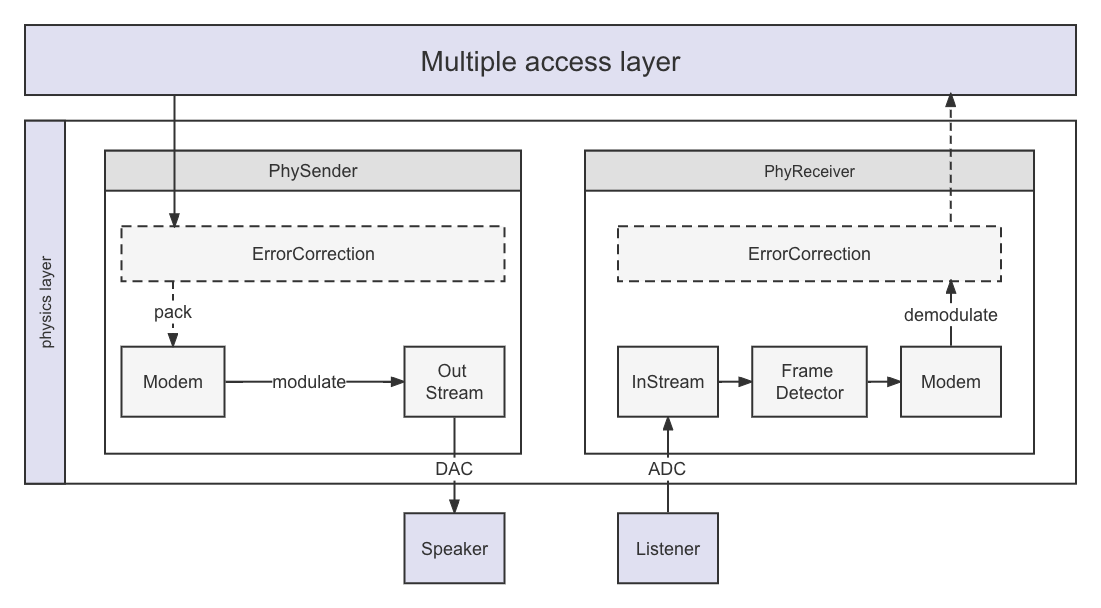
\includegraphics[width=\columnwidth]{./figures/Phylayer.png}}
    \caption{the physics layer}
    \label{physics}
  \end{center}
\end{figure}
Bulit on the audio I/O library, PHY enables basic data transmission with no delivery or integrity guarantee.
A PHY frame is a sequence of PCM audio signal samples that represents a chunk of bytes. It is the transmission unit on this layer.
Each frame contains a fixed preamble signal at the beginning for detection as well as synchronization and a payload signal that encodes 0/1 bits.\par
For data transmission, PHY layer constructs a frame from a chunk of bytes and send it through the medium.
For data receiving, PHY layer repeatedly pulls audio samples from the medium and find the beginning of PHY frames.
When a frame is identified, the payload signal is extracted and decoded.
\subsubsection{Preamble Signal Design}
A chirp is a signal whose instaneous frequency increases or decreases with time.
$x_p(t)$ is a linear chirp signal whose lowest and highest instaneous frequency are $f_a$ and $f_b$ respectively.
\[
  x_p(t) = \begin{cases}
    \pi \dfrac{f_b-f_a}{T} t^2       + 2\pi f_a t     & t\in [0,T]  \\
    \pi \dfrac{f_a-f_a}{T} {(t-T)}^2 + 2\pi f_b (t-T) & t\in [T,2T] \\
  \end{cases}
\]
Chirp signal has a distinct frequency-domain feature so it won't interfere background nosie and the carrier wave.
Auto-correlation energy peak detection is used to find the starting position of the preamble signal which is followed by the payload signal.

\subsubsection{Modulation and Demodulation}
In order to transmit and receive digital signals, a modulation scheme has to be implemented.
Air and audio cabel are media of different characteristic, so they need different modulation schemes.\par
For wireless scenario, background noisy is strong from 0Hz to 6000Hz,
so a passband modulation scheme
combining binary phase shift keying (BPSK) and orthogonal frequency-division multiplexing (OFDM)
is used.
BPSK encodes bits with phase changes:
\begin{align*}
  x_0(t) & =\sin(2\pi f\, t)                       \\
  x_1(t) & =\sin(2\pi f\, t + \pi) = -\sin(2\pi f) \\
\end{align*}
are used to represent 0 bit and one 1 respectively.
To recover a bit from audio signal, consider the dot products $\langle x_0(t),x_0(t)\rangle$ and $\langle x_0(t),x_1(t) \rangle$:
\begin{align*}
  \int_a^b \left( x_0(t)\cdot x_0(t) \right) \mathrm{d}t & =  \int_a^b x_0^2(t) \mathrm{d}t > 0 \\
  \int_a^b \left( x_0(t)\cdot x_1(t) \right) \mathrm{d}t & = -\int_a^b x_0^2(t) \mathrm{d}t < 0 \\
\end{align*}
A zero bit is produced if the dot of the received samples and samples of $x_0(t)$ is positive, otherwise a one bit is produced.\par
To increase the utilization rate of the spectrum, OFDM of $N=64$ is introduced.
However, unlike radio medium, transmitting real part and imaginary part of a complex number simultaneously is not possible,
so only half of the frequency channels can be used to encode bits.
Also, several channels of extremely low and high frequency are not usable as background noise is too strong.\par
As for cabel-connected scenario, baseband transmission is feasible as low frequency background noise no longer exists.
4B5B + non-return to zero inverted(NRZI) enables higher bandwidth and lower error rate.

\subsection{Medium Access Control sublayer}
The medium access control layer regulates access to the shared medium and implements error detection and retransmission mechanism.
\begin{figure}[h]
  \begin{center}
    \centerline{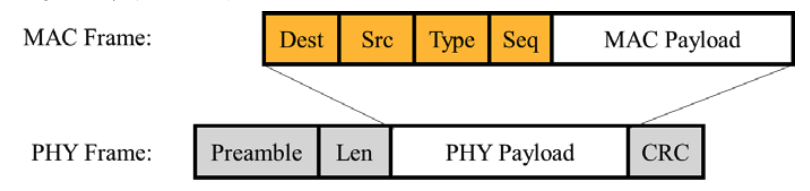
\includegraphics[scale=0.4]{./figures/macpacket.png}}
    \caption{the MAC frame}
    \label{macpacket}
  \end{center}
\end{figure}
A MAC frame is placed in the payload field of a PHY frame so that it can be sent/received through PHY layer.

\subsubsection{CSMA/CA}
\begin{figure}[h]
  \begin{center}
    \centerline{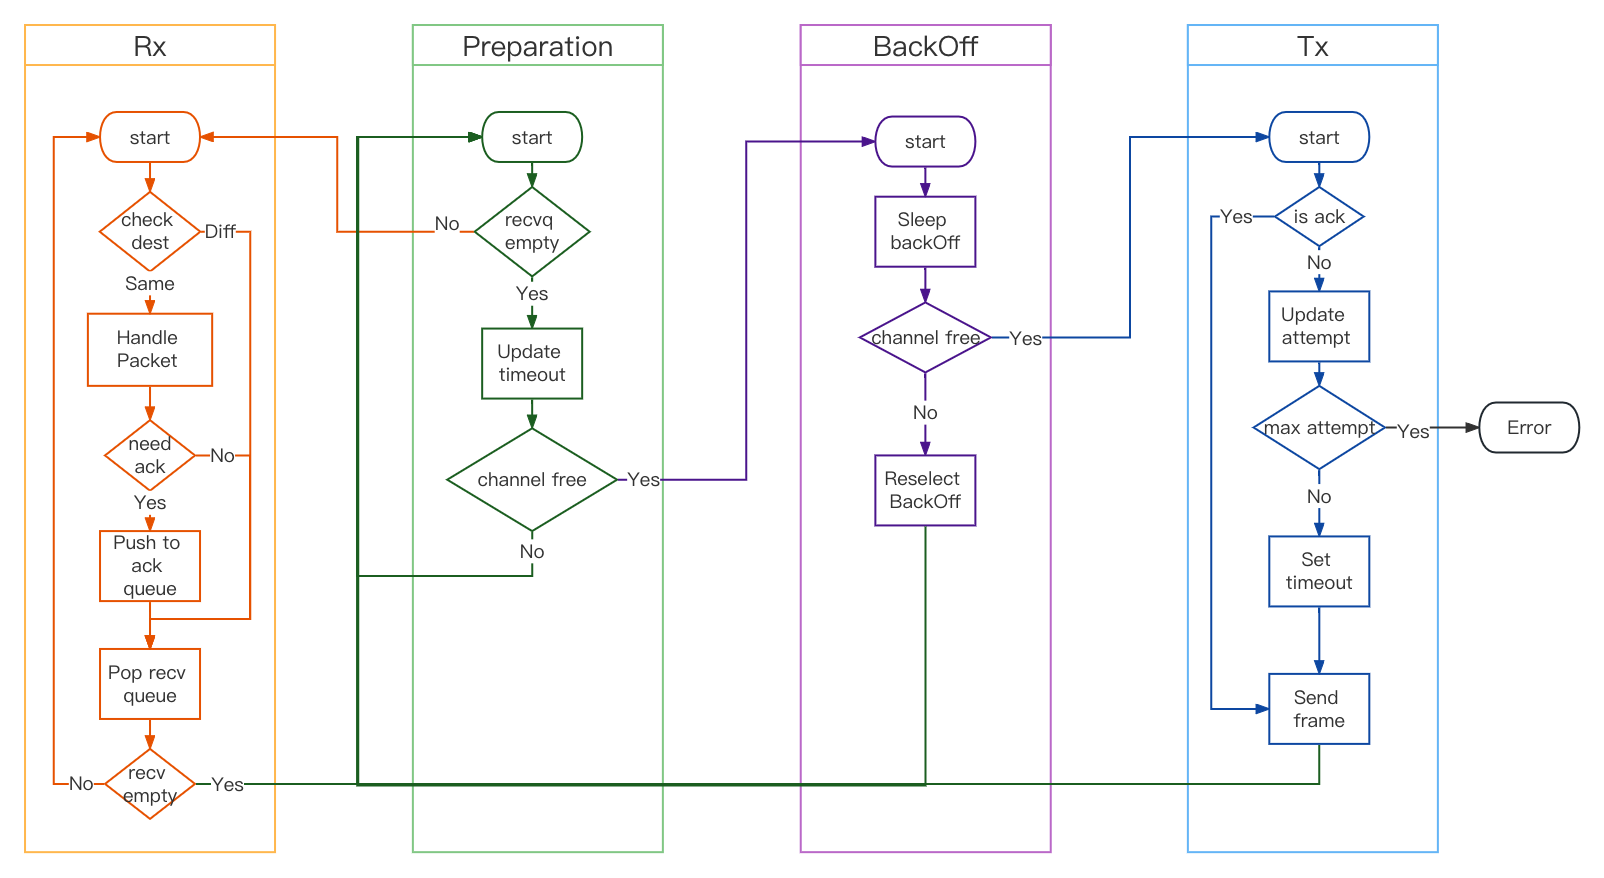
\includegraphics[width=\columnwidth]{./figures/CSMA.png}}
    \caption{the CSMA/CA procdcure}
    \label{csma}
  \end{center}
\end{figure}
We implemented \emph{Carrier Sense Multiple Access with Collision Avoidance (CSMA/CA)}. Each device will listen to the channel before transmitting. If the channel is busy, the device will wait for a random time and then try to resend the data. The time is chosen by the exponential backoff algorithm. The state transition diagram is shown in Figure~\ref{csma}

\subsubsection{Time-division multiplexing MAC}
Due to the latency of the audio driver, the original CSMA/CA suffers from the remote collision. We also implemented Time-division multiplexing MAC., which allocates a fixed time slot for the device to send and receive the packets. We can use the pre-existing Network Time Protocol to synchronize the time of local nodes.

\subsubsection{Sequence Number and Error Detection}
The sequence number and CRC checksum fields are used to drop out-of-order packets and corrupted packets.
A sliding window transmission control is implemented to provide reliable in-order data transmission.

